%%%%%%%%%%%%%%%%%%%%%%%%%%%%%%%%%%%%%%%%%%%%%%%%%%%%%%%
% A template for Wiley article submissions.
% Developed by Overleaf. 
%
% Please note that whilst this template provides a 
% preview of the typeset manuscript for submission, it 
% will not necessarily be the final publication layout.
%
% Usage notes:
% The "blind" option will make anonymous all author, affiliation, correspondence and funding information.
% Use "num-refs" option for numerical citation and references style.
% Use "alpha-refs" option for author-year citation and references style.

\documentclass[alpha-refs]{wiley-article}

% Add additional packages here if required
\usepackage{multirow}
\usepackage{gensymb}

% Update article type if known
\papertype{Original Article}
% Include section in journal if known, otherwise delete
%\paperfield{Journal Section}

\title{Should analog methods use ERA5 for statistical precipitation downscaling? }

% List abbreviations here, if any. Please note that it is preferred that abbreviations be defined at the first instance they appear in the text, rather than creating an abbreviations list.
\abbrevs{AMs, analog methods; ....}

% Include full author names and degrees, when required by the journal.
% Use the \authfn to add symbols for additional footnotes and present addresses, if any. Usually start with 1 for notes about author contributions; then continuing with 2 etc if any author has a different present address.
\author[1]{Pascal Horton}

% Include full affiliation details for all authors
\affil[1]{Oeschger Centre for Climate Change Research and Institute of Geography, University of Bern, Bern, Switzerland}

\corraddress{Pascal Horton, Oeschger Centre for Climate Change Research and Institute of Geography, University of Bern, 3012 Bern, Switzerland}
\corremail{pascal.horton@giub.unibe.ch}

%\presentadd[\authfn{2}]{Department, Institution, City, State or Province, Postal Code, Country}

%\fundinginfo{Funder One, Funder One Department, Grant/Award Number: 123456, 123457 and 123458; Funder Two, Funder Two Department, Grant/Award Number: 123459}

% Include the name of the author that should appear in the running header
\runningauthor{P. Horton}

\begin{document}

\maketitle

\begin{abstract}
Statistical downscaling techniques that are of the perfect prognosis type rely on statistical relationships established between observational data for both predictands and predictors. Predictors are often retrieved from reanalyses, which are considered as pseudo-observations. The impact of the choice of a reanalysis dataset on the skill of the downscaling method is often overlooked as global reanalyses are frequently assumed to be equivalent for the last decades and for data-rich regions such as Europe. However, it was recently shown that the selection of a reanalysis dataset has an impact on the skill of the method that can be even higher than the selection of the predictor variables. The obvious general tendency is that reanalyses that are processed by more recent atmospheric models and that assimilate more data perform better. 

Following the recent release of ERA5, this work aims at assessing the extent of the potential gain compared to other global reanalyses, including its predecessor, ERA-interim. The assessment was carried out using six variants of analog methods, which are statistical downscaling techniques, to predict the daily precipitation at 301 stations in Switzerland. Among the ten reanalyses that were compared, ERA5 ended up in the best performing datasets, and was the best choice for 50\% of the stations in average across the different analog methods. 

However, ERA5 is distributed with a high spatial resolution (0.25\degree), which turned out to be not relevant for analog methods, and which can even be a trap for simple calibration techniques. Indeed, the domains over which the predictor fields are compared need to be optimized, and high-resolution grids come along with numerous sub-optimal local minima. Besides the risk of poorly-calibrated domains, the high resolution also involves much higher computational time for no gain in skill, as long as the predictors are at synoptic scale.


% Please include a maximum of seven keywords
\keywords{reanalyses, ERA5, statistical downscaling, analog method, precipitation, Switzerland}
\end{abstract}

\section{Introduction}

Analog methods (AMs), which are part of the statistical downscaling techniques, aim at predicting local meteorological variables, often daily precipitation, based on large-scale predictors. AMs rely on the hypothesis that similar synoptic situations are likely to result in similar local effects, plus a certain variability that is not explained by the considered predictors \citep{Lorenz1969}. To account for this unexplained variability, an ensemble of analog situations is considered, providing an statistical prediction in the form of an empirical conditional distribution made of the corresponding observed predictand values. Multiple variants of the AM exist, eventually with different structures and approach, but mainly with different selections of predictors.

AMs are most often developed in a perfect prognosis framework \citep{Rummukainen1997, Maraun2010}, where the relationship is calibrated between large-scale and local-scale observations. In this context, global reanalyses are the datasets of choice for the large-scale variables as they provide multivariate gridded outputs that are physically consistent and available all around the globe \citep{Gelaro2017}. There are globally two main types of reanalysis products: those that aim for homogeneity over a long period -- starting at the beginning of the 20th century -- and thus assimilate surface data only, and those that aim for accuracy over a more recent period and that assimilate a maximum of observations, including multiple satellite products. The accuracy of the reanalyses depends on the quality of the model physics and that of the analysis process, thus on the quantity and quality of the assimilated observations \citep{Dee2011a}.

The choice of a reanalysis dataset to be used in an AM can be driven by the context of the application, for example if it requires to cover the 20th century or to be used in an operational context, with the target situation being provided by a NWP model. In the first case, ECMWF twentieth century reanalyses \citep[ERA-20C or CERA-20C --][]{Poli2016, Laloyaux2016} or the Twentieth Century Reanalysis \citep[20CR --][]{Compo2011} produced by NOAA can be used \citep[for example,][]{Kuentz2015, Caillouet2016, Brigode2016, Bonnet2017}. In the second case, one should prefer a reanalysis that is produced by the same model as the operational forecast to reduce the inter-models biases. However, in many cases, the selection of the reanalysis is arbitrary and might be driven by a preference for the local provider. 

NCEP/NCAR Reanalysis 1 \citep[NR-1 --][]{Kalnay1996, Kistler2001} and NCEP/DOE Reanalysis 2 \citep[NR-2 --][]{Kanamitsu2002} were used in many applications of AMs \citep{Timbal2003, Bontron2004, Wetterhall2005a, Gangopadhyay2005, Altava-Ortiz2006, Barrera2007, Cannon2007, Matulla2007, Bliefernicht2007, Maurer2008, BenDaoud2009, Wu2012, Marty2012, Teng2012, Horton2012, Yiou2014}. ERA-40 \citep{Uppala2005}, produced by ECMWF, has also been used substantially \citep {BenDaoud2009, Willems2011b, JakobThemessl2011a, BenDaoud2011, Turco2011a, Franke2011, Pascual2012b, Schenk2012, Ribalaygua2013a, Osca2013, Radanovics2013, Martin2014b, Chardon2014, BenDaoud2016}. Its sucessor, ERA-Interim \citep[ERA-INT --][]{Dee2011a}, has been used by \cite{Raynaud2016b}. NASA's Modern-Era Retrospective Analysis for Research and Applications \citep[MERRA -- ][]{Rienecker2011} has been used by \citet{Vanvyve2015}. The Japanese products, the Japanese 55-year Reanalysis \citep[JRA-55 --][]{Kobayashi2015, Harada2016} and its conventional-only JRA-55 Conventional \citep[JRA-55C --][]{Kobayashi2014}, were not used in AMs to the author knowledge. Newer products, such as NCEP's the Climate Forecast System Reanalysis \citep[CFSR --][]{Saha2010a} or MERRA version 2 \citep[MERRA-2 -- ][]{Gelaro2017} are not much used yet in AMs. One can often observe a lag between the release of a new reanalysis dataset and its adoption in AMs.

Most applications of AMs are based on a single reanalysis dataset and the impact of this choice is overlooked. \citet{BenDaoud2009} compared NR-1 to ERA-40 and found no significant difference for the predictors considered. Later, \citet{Dayon2015} compared NR-1, MERRA, ERA-INT and 20CR and found out that the choice of the reanalysis dataset has a non-negligible impact on the performance of the AMs that can even be greater than the choice of the predictor variables. They concluded that the role of the reanalyses should not be underestimated. Such an influence has also been observed for other statistical downscaling methods \citep[e.g.][]{Koukidis2009}. \citet{Horton2018b} compared ten global reanalyses and concluded that the impact of the dataset on the results of the AM are significant. The conclusion was similar to that of \citet{Dayon2015}, in that the influence of the reanalysis can be bigger than that of the predictors selection. Some recommendations were established to guide for the choice of the reanalysis depending on the period and the predictors of interest. Globally, more recent products that assimilate more data show better skills \citep{Horton2018b}. In that respect, the recent release of ERA5 \citep{Hersbach2019} raises the question of how better it can be for AMs compared to its predecessor ERA-Interim, and what are the benefits and eventual pitfalls of its higher spatial and temporal resolutions.

ERA5 was compared to nine other global reanalyses for seven AMs at 301 stations in Switzerland. The data and methods are described in section \ref{sec:data_methods}. The impact of the skill is presented in section \ref{sec:results_skill}, the spatial resolution is assessed in section \ref{sec:results_hires}, and the similarity to other reanalyses is presented in section \ref{sec:results_shared_dates}. The conclusions (section \ref{sec:conclusion}) summarize the key findings.


\section{Data and methods}
\label{sec:data_methods}

\subsection{Reanalyses}
\label{sec:reanalyses}

The present work aims at comparing ERA5 \citep{Hersbach2019} to other global reanalyses, which characteristics are provided in Table \ref{table:datasets}. The three first reanalyses are surface-input \citep{Fujiwara2017} products that assimilate surface data only, but cover a long period, typically the 20th century. NOAA produced the Twentieth Century Reanalysis \citep[version 2c, 20CR-2c --][]{Compo2011} which only assimilates surface pressure data and uses observed monthly sea-surface temperature and sea-ice distributions as boundary conditions. The European Centre for Medium-Range Weather Forecasts (ECMWF) developed two products using surface input only: ERA-20C \citep{Poli2016} that assimilates marine wind observations and is forced by sea surface temperature, sea ice cover, atmospheric composition changes, and solar forcing, and CERA-20C \citep{Laloyaux2018a}, which has an additional coupling to the ocean and was produced by a more recent version of the IFS model.

The other reanalyses are full-input products as they assimilate all available data, including satellite data \citep{Fujiwara2017}. The NCEP/NCAR Reanalysis I \citep[NR-1 --][]{Kalnay1996, Kistler2001} was the first global reanalysis, followed by the NCEP/DOE Reanalysis 2 \citep[NR-2 --][]{Kanamitsu2002} that fixed some identified problems. The Climate Forecast System Reanalysis \citep[CFSR --][]{Saha2010a} is the most recent reanalysis by NCEP. The Japanese 55-year Reanalysis \citep[JRA-55 --][]{Kobayashi2015, Harada2016} is produced by the Japan Meteorological Agency (JMA). Its version using conventional data only, JRA-55 Conventional \citep[JRA-55C --][]{Kobayashi2014}, was not considered in this work as it provides similar results as JRA-55 \citep{Horton2018b}. NASA's Global Modeling and Assimilation Office (GMAO) released the Modern-Era Retrospective Analysis for Research and Applications, version 2 \citep[MERRA-2 -- ][]{Gelaro2017}, which is an improvement of the first MERRA reanalysis \citep{Rienecker2011}. Finally, the predecessor of ERA5, ERA-Interim \citep[ERA-INT --][]{Dee2011a}, was also considered.

ERA5 \citep{Hersbach2019} is meant to replace ERA-Interim. It profits from multiple improvements to the Integrating Forecasting System (IFS), in terms of model physics, core dynamics, and data assimilation \citep{Hersbach2019}. It provides more outputs, with higher temporal (hourly) and spatial (0.28\degree; 31~km) resolutions. The use of a 10-member ensemble of data assimilations at a lower spatial and temporal resolution allows providing an estimate of the uncertainty. ERA5 assimilates significantly more data than ERA-Interim, such as ground-based radar and new satellite sensors, and uses improved observation operators, which allows to better compare model outputs and observations. Additionally, it indirectly profits from improvements of historical observations, both for conventional and satellite data \citep{Hersbach2019}. ERA5 is also more appropriate for climate analyses as it relies on suitable radiative forcing and boundary conditions (e.g. changes in greenhouse gases, aerosols, SST, and sea ice).


\begin{table}[bt]
	\caption{Assessed reanalysis datasets with their respective properties, sorted by type and model age.}
	\small
	\begin{threeparttable}
	\begin{tabular}{lllllll}
		\hline
		\headrow
		\thead{Name} & \thead{Institution} & \thead{Coverage} & \thead{Output} & \thead{Model resolution \& age} & \thead{Input} & \thead{Assimilation}\\
		\hline 
		\textbf{20CR-2c} & NOAA-CIRES & 1851 -- 2014 & 2\degree x 2\degree & T62 ($\sim$1.88\degree), L28, 2008 & surface  & EnKF\\
		\textbf{ERA-20C} & ECMWF & 1900 -- 2010 & 1\degree x 1\degree & TL159 ($\sim$1.13\degree), L9, 2012 & surface  & 4D-Var\\
		\textbf{CERA-20C} & ECMWF & 1901 -- 2010 & 1\degree x 1\degree & T159 ($\sim$1.13\degree), L91, 2016 & surface & 4D-Var\\
		\hline 
		\textbf{NR-1} & NCEP, NCAR & 1948 -- present & 2.5\degree x 2.5\degree & T62 ($\sim$1.88\degree), L28, 1995 & full & 3D-Var\\
		\textbf{NR-2} & NCEP, DOE & 1979 -- present & 2.5\degree x 2.5\degree & T62 ($\sim$1.88\degree), L28, 2001 & full  & 3D-Var\\
		\textbf{CFSR} & NCEP & 1979 -- present & 0.5\degree x 0.5\degree & T382 ($\sim$0.31\degree), L64, 2009 & full  & 3D-Var\\
		\textbf{JRA-55}  & JMA & 1958 -- present & 1.25\degree x 1.25\degree & TL319 ($\sim$0.36\degree), L60, 2009 & full  & 4D-Var\\
		%\textbf{JRA-55C}  & JMA & 1958 -- 2015 & 1.25\degree x 1.25\degree & TL319 ($\sim$0.36\degree), L60 & 2009 & conventional  & 4D-Var\\
		\textbf{MERRA-2} & NASA GMAO & 1980 -- present & 0.625\degree x 0.5\degree & 0.625\degree x 0.5\degree, L72, 2014 & full  & 3D-Var\\
		\textbf{ERA-INT} & ECMWF & 1979 -- 2017 & 0.75\degree x 0.75\degree & TL255 ($\sim$0.70\degree), L60, 2006 & full  & 4D-Var\\
		\textbf{ERA5} & ECMWF & 1950* -- present & 0.25\degree x 0.25\degree & T639 ($\sim$0.28\degree), L137, 2016 & full  & 4D-Var\\
		\hline 
	\end{tabular} 

	\begin{tablenotes}
		\item *expected to be available in 2020. The available period starts in 1979 at time of writing.
		%\item JKL, just keep laughing; MN, merry noise.
	\end{tablenotes}
	\end{threeparttable}
	\label{table:datasets}
\end{table}

%ERA5 strengths compared to ERA-Interim
%Much higher spatial and temporal resolution
%Information on variation in quality over space and time
%Much improved troposphere
%Improved representation of tropical cyclones
%Better global balance of precipitation and evaporation
%Better precipitation over land in the deep tropics
%Better soil moisture
%More consistent sea surface temperature and sea ice

\subsection{Precipitation dataset}
\label{sec:precipitation}

The local variable to be predicted is here daily precipitation totals (06:00~h~UTC to 06:00~h~UTC the following day) at 301 stations of the MeteoSwiss network in Switzerland (Fig. \ref{fig:stations}), with a good coverage of the 1981--2010 period. The 30-year precipitation dataset was divided into a calibration period (CP) and an independent validation period (VP), which was evenly distributed over the entire series (1 year out of every 5; total of 6 years). The archive period (AP), where the analogue dates are being retrieved, is the same as the CP -- also with the VP being excluded -- with an additional exclusion of $\pm30$ days around the target date. Results are always presented for the VP.

\begin{figure}
	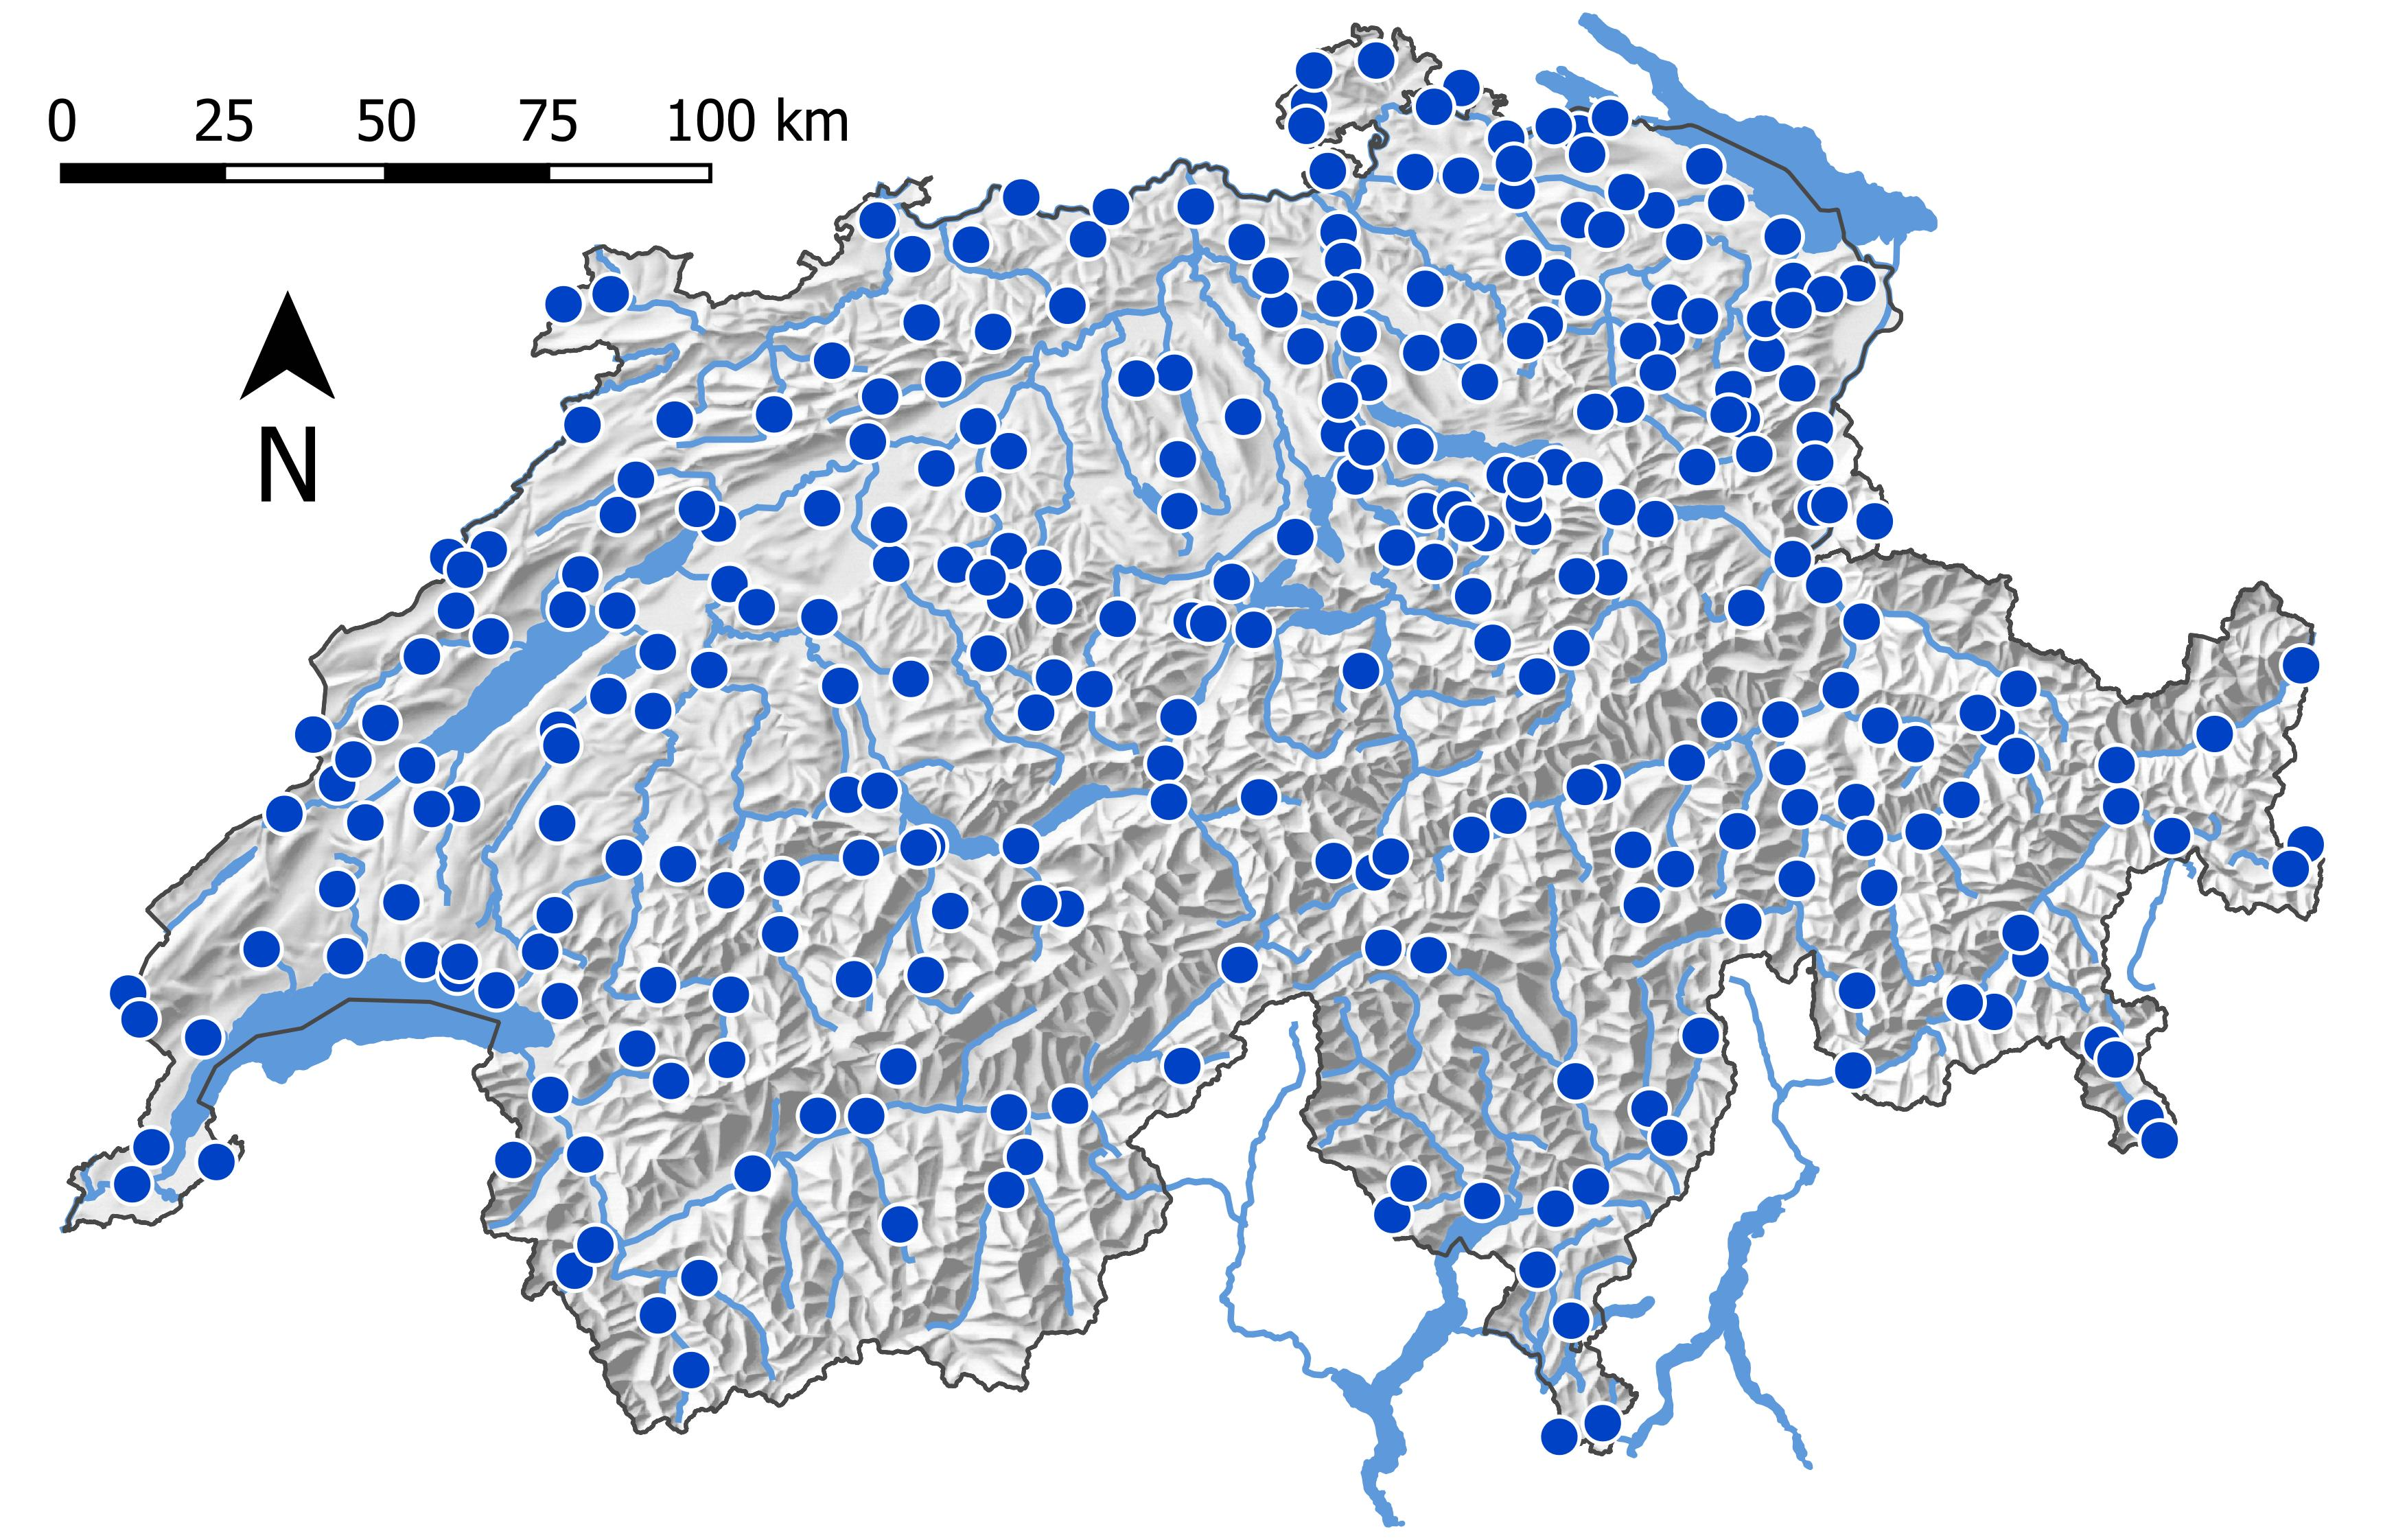
\includegraphics[width=70mm]{figures/map-stations.jpg}\\
	\caption{Map of the 301 precipitation stations with good data coverage of the period 1981--2010. Background map: \textcopyright\ SwissTopo.}
	\label{fig:stations}
\end{figure}


\subsection{Analog methods}
\label{sec:ams}

Most variants of the AM from \cite{Horton2018b} were considered (Table \ref{table:methods}). These AMs have different degrees of complexity, but they all start with a preselection in order to cope with seasonality. A commonly used preselection is based on the dates (PC: preselection on calendar basis in Table \ref{table:methods}) as candidate situations are extracted from the archive for a period of 120~days centered around the target date. To allow for a more dynamic approach, \citet{BenDaoud2016} based this preselection on the similarity of air temperature (T) at 925~hPa and 600~hPa at the nearest grid point. An undesired mixing of spring and autumn situations is discussed in \citet{Caillouet2016}. 

\begin{table*}[t]
	\caption{Analogue methods considered in the study, listed by increasing complexity. The analogy criterion is S1 for SLP and Z and RMSE for the other variables.}
	\small
	\begin{threeparttable}
		\begin{tabular}{llllll}
			\hline
			\headrow
			\thead{Method} & \thead{P0} & \thead{L1} & \thead{L2} & \thead{L3} & \thead{Reference} \\ 
			\hline 
			\multirow{2}{*}{\textbf{2Z}} & \multirow{2}{*}{PC} & Z1000@12h &&& \multirow{2}{*}{\citealp{Bontron2004}} \\
			&& Z500@24h &&& \\
			\hline 
			\multirow{4}{*}{\textbf{4Z}} & \multirow{4}{*}{PC} & Z1000@06h &&& \multirow{4}{*}{\citealp{Horton2018a}} \\
			&& Z1000@30h &&& \\
			&& Z700@24h &&& \\
			&& Z500@12h &&& \\
			\hline 
			\multirow{2}{*}{\textbf{2Z-2MI}} & \multirow{2}{*}{PC} & Z1000@12h & \multirow{2}{*}{MI850@12+24h} && \multirow{2}{*}{\citealp{Bontron2004}} \\
			&& Z500@24h &&& \\
			\hline 
			\multirow{4}{*}{\textbf{4Z-2MI}} & \multirow{4}{*}{PC} & Z1000@30h &&& \multirow{4}{*}{\citealp{Horton2018a}}\\
			&& Z850@12h & MI700@24h && \\
			&& Z700@24h & MI600@12h && \\
			&& Z400@12h &&& \\
			\hline 
			\multirow{2}{*}{\textbf{PT-2Z-4MI}} & T925@36h & Z1000@12h & MI925@12+24h && \multirow{2}{*}{\citealp{BenDaoud2016}} \\
			& T600@12h & Z500@24h & MI700@12+24h && \\
			\hline 
			\multirow{2}{*}{\textbf{PT-2Z-4W-4MI}} & T925@36h & Z1000@12h & \multirow{2}{*}{W850@06-24h} & MI925@12+24h & \multirow{2}{*}{\citealp{BenDaoud2016}} \\
			& T600@12h & Z500@24h && MI700@12+24h & \\
			\hline 
		\end{tabular} 
		
		\begin{tablenotes}
			\item P0, preselection (PC: $\pm 60$ days around the target date); L1, L2 and L3, subsequent levels of analogy.
			\item Z, geopotential height; T, air temperature; W, vertical velocity; MI, moisture index (product of the relative humidity at the given pressure level and the total water column).
		\end{tablenotes}
	\end{threeparttable}
	\label{table:methods}
\end{table*}

All considered AMs have a first level of analogy on the atmospheric circulation, using the geopotential height (Z) at different pressure levels and time as predictor. This analogy is quantified by the S1 criterion \citep[Eq.\ \ref{eq:S1}, ][]{Teweles1954, Brown2012}, which is a comparison of gradients over a selected (calibrated) domain. The objective is to compare the atmospheric flow and not the absolute values of the respective fields. The values of the criterion processed for different levels/hours are here averaged into a single value for a given candidate date. More advanced approaches introduce a weighting between these diverse components \citep{Horton2017a}.

\begin{equation}
	\label{eq:S1}
	S1=100 \frac{\sum_{i} \vert \Delta\hat{z}_{i} - \Delta z_{i} \vert}{\sum_{i} \max\left\lbrace \vert \Delta\hat{z}_{i} \vert; \vert \Delta z_{i} \vert \right\rbrace }
	% use \displaystyle to max sum sign larger
\end{equation}
where $\Delta \hat{z}_{i}$ is the geopotential height gradient between the \textit{i}-th pair of points for the target day, and $\Delta z_{i}$ is the corresponding observed geopotential height gradient for the candidate situation. The smaller the values S1 are, the more similar the pressure fields.

The most simple method, 2Z, is based only on the analogy of the atmospheric cirulation, using the geopotential height at 1000~hPa and 500~hPa, \citep{Bontron2004}. The most similar $N_{1}$ dates, with the lowest values of S1, are selected as analogues to the target date. The daily precipitation that was measured at these $N_{1}$ dates then provides the empirical conditional distribution, considered as the probabilistic prediction for the target date.

The second method, 4Z, is also based on geopotential height only, but using four combinations of pressure levels and temporal windows \citep{Horton2018a}. This method is here considered as a simplified version of a more complex method elaborated by genetic algorithms. It was found that using four geopotentiel height is more informative than using only two.

Then, the next three methods (2Z-2MI, 4Z-2MI, PT-2Z-4MI, Table \ref{table:methods}) add a second level of analogy to subsample from the first level, based on moisture variables. The predictor considered here is a moisture index (MI), which is the product of the total precipitable water (TPW) and the relative humidity (RH) and was introduced by \citet{Bontron2004}. This predictor is assessed using the root mean square error (RMSE) criterion. The 2Z-2MI method \citep{Bontron2004} considers this index at 850~hPa for two different hours (+12 h and +24 h). The 4Z-2MI method \citep{Horton2018a}, derived from optimizations with genetic algorithms, consider the 600~hPa and 700~hPa levels, but with a change in the selected levels of the geopotential height compared to 4Z. The 4Z-2MI method \citep{BenDaoud2016} considers the moisture index at 700~hPa and 925~hPa, both at +12 h and +24 h.

Finally, the most complex method, PT-2Z-4W-4MI, also named "SANDHY" for Stepwise Analogue Downscaling method for Hydrology \citep{BenDaoud2016, Caillouet2016}, adds an intermediate level of analogy, before the moisture predictors, based on the vertical velocity (W) at 850~hPa. It was primarily developed for large and relatively flat/lowland catchments in France (Sa\^{o}ne, Seine).


\subsection{Calibration of the methods} %\subsubsection?
\label{sec:calibration}

The CRPS \citep[Continuous Ranked Probability Score,][]{Brown1974, Matheson1976, Hersbach2000} is often used as objective function, and allows evaluating the predicted cumulative distribution provided by the analogs compared to the single observed value at the target date. Its skill score expression, the CRPSS (Continuous Ranked Probability Skill Score), was used here, using the climatological distribution of precipitation as the reference. It allows a better comparison between stations as it partly takes into account the differences in climatology. The CRPSS is expressed as follows \citep{Bradley2011}:

\begin{equation}
	\label{eq:CRPSS}
	CRPSS = 1-\frac{\overline{CRPS}}{\overline{CRPS}_{clim}}
\end{equation}
where $CRPS_{clim}$ is the CRPS value for the climatological distribution. A better prediction is characterized by an increase in CRPSS.

The methods were here calibrated using the semi-automatic sequential procedure developed by \citet{Bontron2004} and also used in \citet{Radanovics2013} and \citet{BenDaoud2016}. A detailed description can also be found in \citet{Horton2019}. It allows the calibration of the spatial windows on which the predictors are compared (specific to each level of analogy) and of the number of analog dates to select at the different levels of analogy. The AtmoSwing software \citep{Horton2019} was used to perform this calibration independently for every station, method, and reanalysis. The calculations were performed on a HPC cluster at the University of Bern. 

After the initial calibration of all AMs for ERA5, some issues were identified due to the presence of local minimas for the spatial windows in the high resolution grid. The procedure was then restarted using an improvement of the semi-automatic procedure, named classic+ \citep{Horton2019}, which allows additional moves in the calibration of the spatial windows and thus allows escaping local minimas. This issue is presented and discussed in section \ref{sec:results_hires}.


\section{Results}
\label{sec:results}

The results are provided for the VP (independent validation period, section \ref{sec:precipitation}). All reanalyses were used at their highest available spatial resolution and at a 6-hrly time step. The impact of the spatial resolution is analyzed in section \ref{sec:results_hires}.

\subsection{Impact on the skill}
\label{sec:results_skill}

The skill score of the different methods and reanalyses are shown in Fig. \ref{fig:comparison_values}. As discussed in \citet{Horton2018b}, there are clear differences between methods, with more complex AMs generally performing better, and also between reanalyses, in favour of modern full-input reanalyses. One can see here that ERA5 is systematically in the best performing reanalyses. When isolating the impact of the reanalysis by removing the influence of the methods and the stations (Fig. \ref{fig:comparison_relative}), the positive contribution of ERA5 to the skill score is even more clear, with the highest difference for the method PT-2Z-4MI. One can also see a clear improvement compared to ERA-INT.

ERA5 was selected as the best reanalysis from a minimum of 34.9\% of the stations for 4Z to a maximum of 78.7\% for PT-2Z-4MI, with an average of about 50\%. When considering the first two ranks, ERA5 was selected from a minimum of 61.8\% of the stations for PT-2Z-4W-4MI to a maximum of 91.7\% for PT-2Z-4MI, with an average of 75\%. There was no specific spatial patterns with respect to which stations performed best with ERA5, such as it was the case with other reanalyses in \citet{Horton2018b}. Also, ERA-INT was not systematically superseded by ERA5, and ERA-INT remained the best choice for some stations and methods. It is thus important to undertake such a comparison on different AMs and multiple stations.


\begin{figure}[bt]
    \centering
    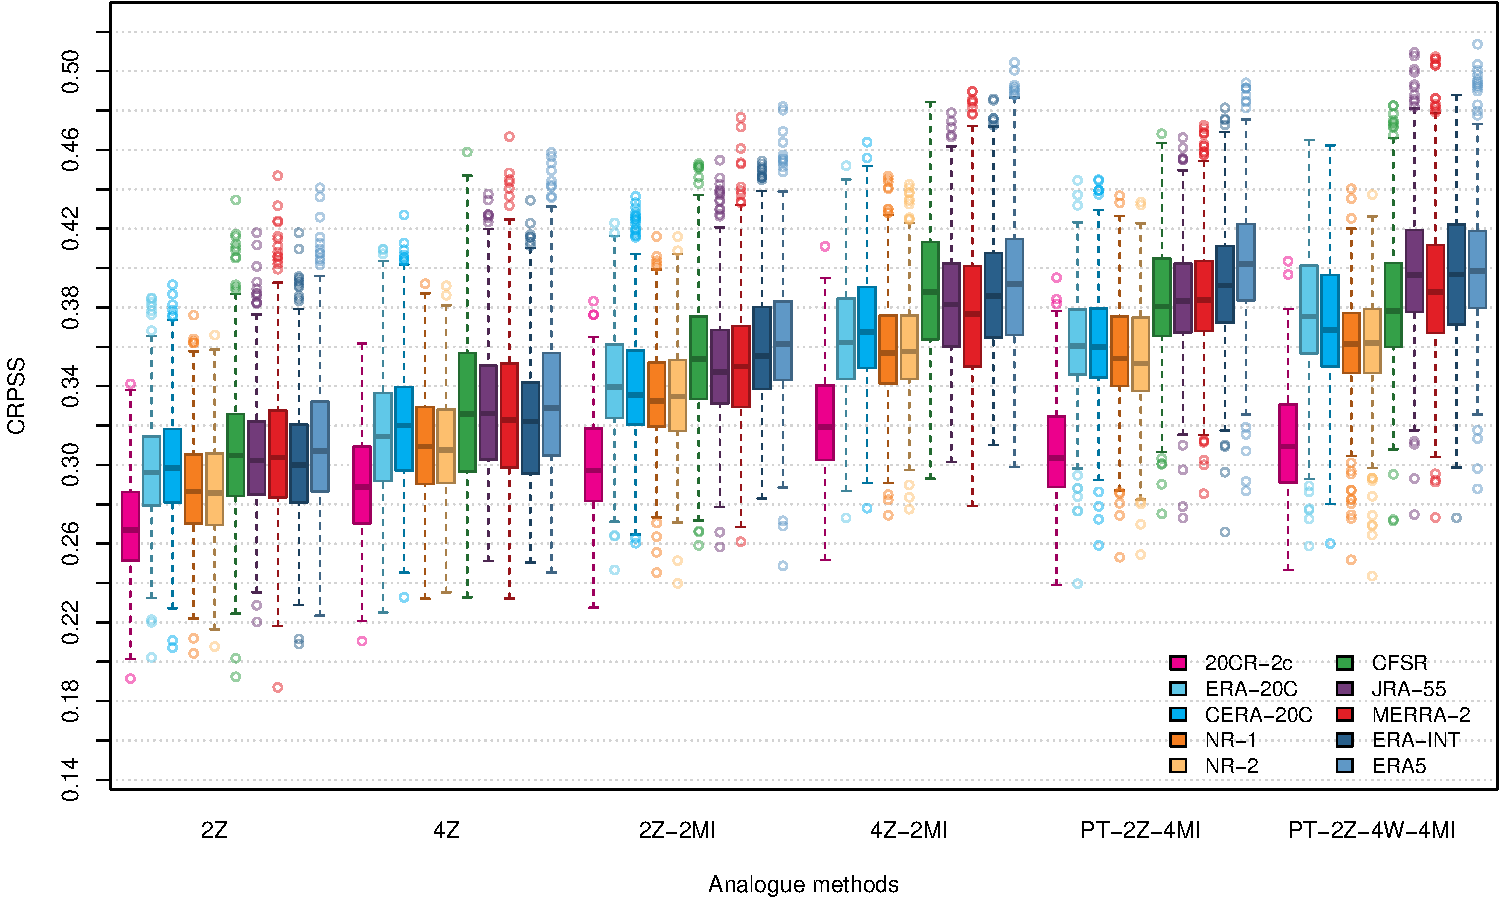
\includegraphics[width=\textwidth]{figures/boxplot-per-method.pdf}
    \caption{CRPSS for all stations, and for all considered AMs and reanalysis datasets on the VP. A higher CRPSS means better performance. The parameters of the AMs were calibrated for every station, every dataset, and every method. The boxes show the 25th, 50th, and 75th percentiles. The whiskers extend to the most extreme data point which is no more than 1.5 times the interquartile range.}
    \label{fig:comparison_values}
\end{figure}

\begin{figure}[bt]
    \centering
    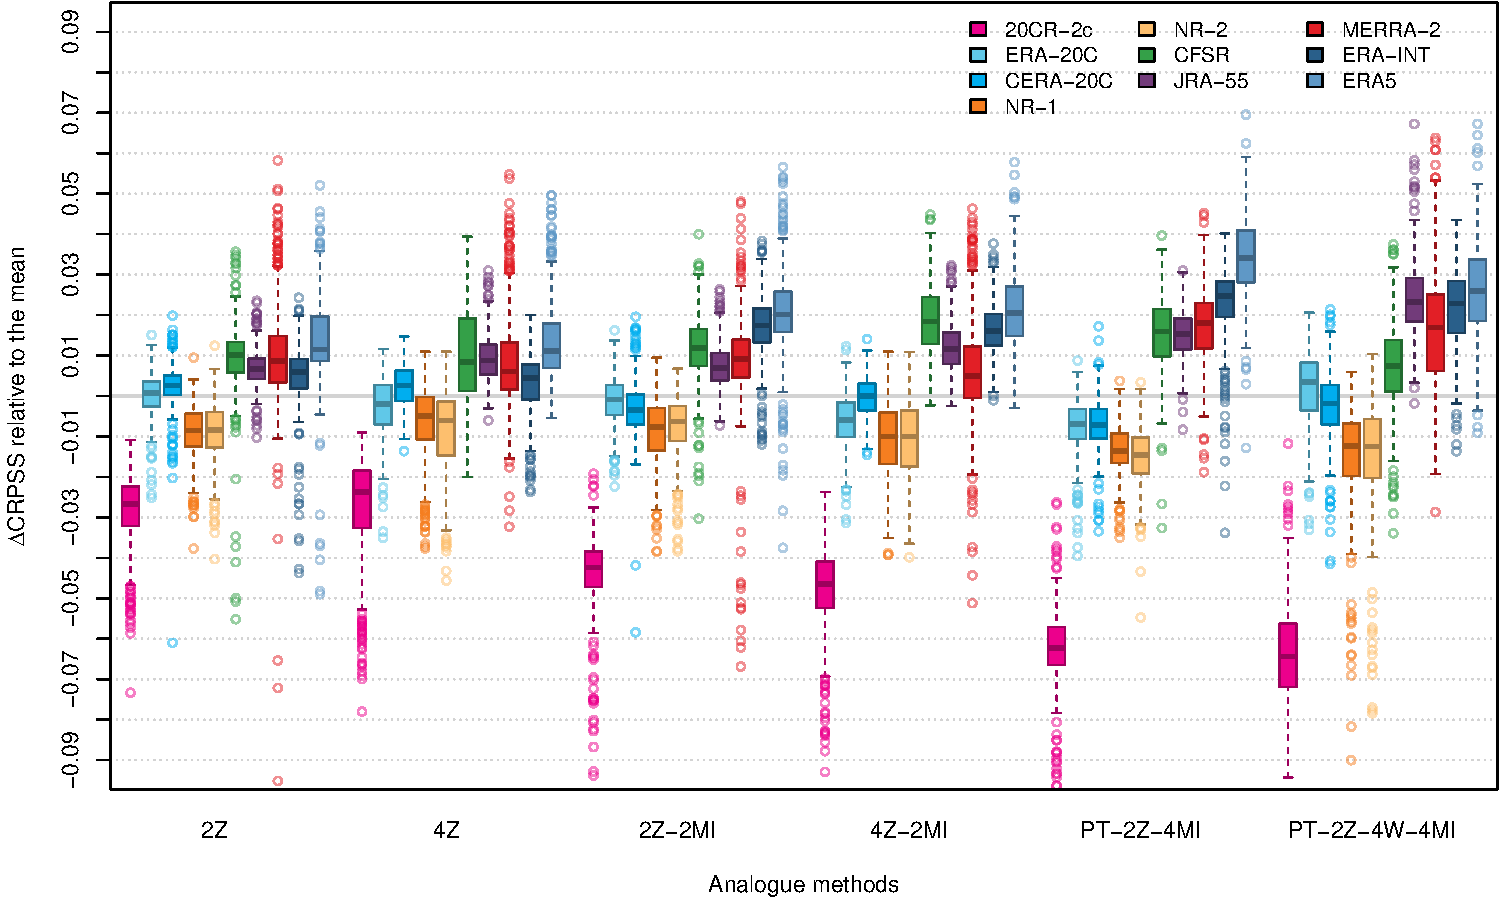
\includegraphics[width=\textwidth]{figures/boxplot-per-method-diff.pdf}
    \caption{Impact of the reanalysis dataset on performance, isolated by processing the improvement in CRPSS for one dataset compared to the mean performance on all datasets, per station and per method. Note that the methods cannot be compared here, only the datasets. Same conventions as Fig. 2.}
    \label{fig:comparison_relative}
\end{figure}


\subsection{High resolution and its pitfalls}
\label{sec:results_hires}

Although the calibrations have been made on a HPC cluster, they ended up to be highly time consuming when using the semi-automatic sequential procedure (classic calibration). The reason being that the process involve first the calculation of a relevance map for each level of analogy, which requires an assessment of every unitary cell of the predictor grid. Then, the spatial window in growing by assessing an extension in every four dimensions and by applying the one with the highest gain. On a high resolution grid, these procedures imply numerous assessments.

\begin{figure}[bt]
	\centering
	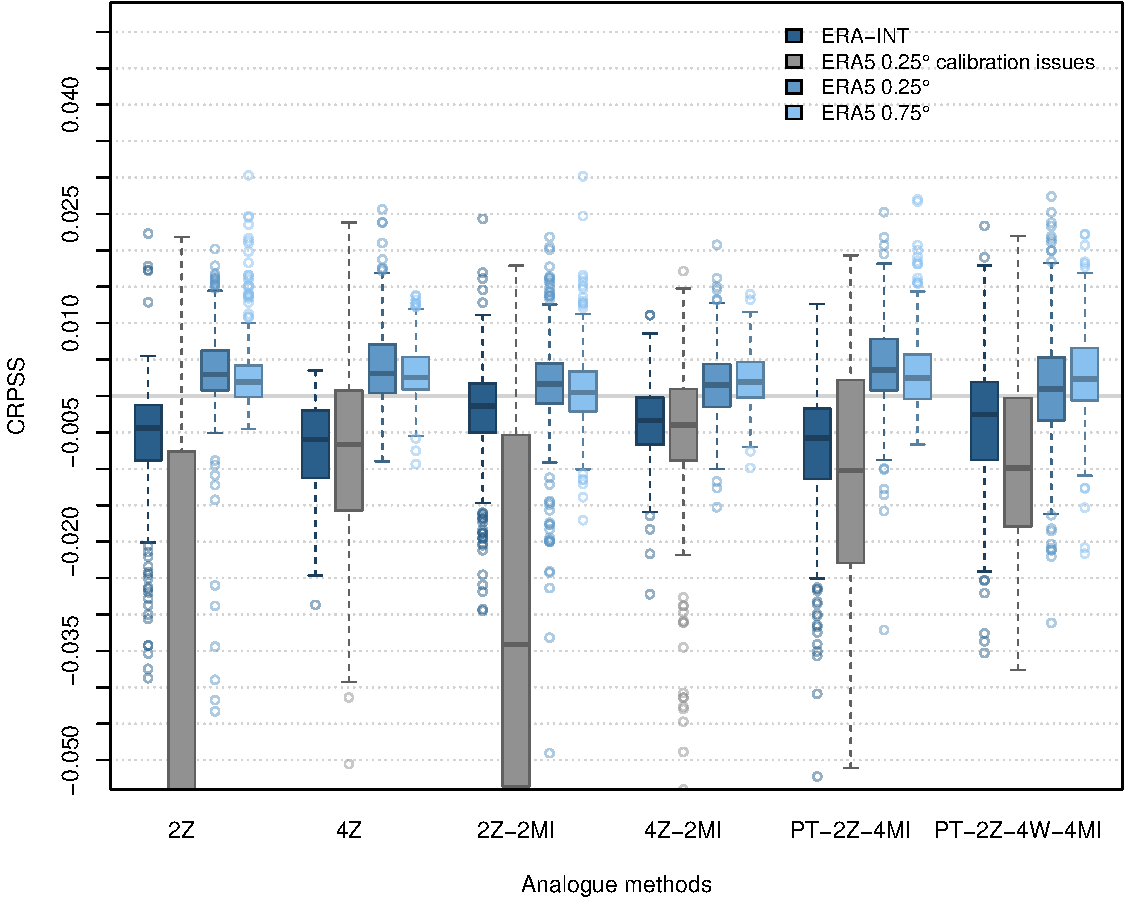
\includegraphics[width=80mm]{figures/boxplot-resol-diff.pdf}
	\caption{Comparison of ERA-INT and ERA5 at 0.25\degree\ and 0.75\degree\ as well as the failed calibration of AMs with ERA5. The impact of the reanalysis on performance has been isolated by processing the improvement in CRPSS for one dataset compared to the mean performance on all datasets (excluding the failed calibration), per station and per method. Same conventions as Fig. 2.}
	\label{fig:resolution}
\end{figure}

When all calibrations were done, the results showed that ERA5 was performing more poorly than ERA-INT (grayed bars in Fig. \ref{fig:resolution}). An investigation of these results showed that the spatial windows did not grow as much as expected and were non optimal. The reason being that the classic calibration got stuck in local minimas during the procedure of the spatial window expansion, as none of the increments in the four directions resulted in a gain in skill. This issue did not happen in a significant way for the other reanalyses and is here due to the very high resolution of ERA5 that can create local minimas that trap the classic calibration. To address this issue, the classic+ calibration (Sect. \ref{sec:calibration}) was then used. It allows additional moves in the growth of the spatial window, including increases of multiple grid points at once to get out of local minimas. The classic+ calibration also ended up to be faster due to its ability to not assess every point of the grid in the calculation of the relevance map. With the advent of high resolution datasets, one should be aware of the potential pitfalls of calibration techniques that were developed on low-resolution datasets.

\citet{Horton2018b} showed that below 1\degree, the spatial resolution of the reanalyses has generally no significant impact on the performance of AMs. ERA5 has the highest spatial resolution among global reanalyses. As the results in Sect. \ref{sec:results_skill} were obtained using the full spatial resolution (0.25\degree), an additional calibration was here performed using the same resolution as ERA-INT (0.75\degree) to quantify the contribution of the resolution in the gain relatively to ERA-INT. Fig. \ref{fig:resolution} shows that degrading the resolution of ERA5 to ERA-INT resolution does not significantly impact the score. Although a higher model resolution is likely contributing to the improvements of ERA5 compared to ERA-INT, the high output resolution has no impact on AMs performance for the prediction of daily precipitation. The gains are likely due to improvements in the forecast model, the assimilation scheme and the assimilated data. While this conclusion is likely valid for predictands that are principally driven by large-scale predictors, it cannot be transposed to all applications. Indeed, when the phenomenon at hand is mainly driven by mesoscale predictors, such as the lightning activity, the output spatial resolution does matter (unpublished results).


\subsection{Shared analog dates}
\label{sec:results_shared_dates}

The use of predictors from different datasets, and of distinct spatial windows, result in a different selection of analog dates. The percentage of identical analogue dates for the different AMs over the VP is shown in Fig. \ref{fig:shared-dates}. This percentage decreases with the complexity of the AM, and range from a maximum of 74\% between NR-1 and NR-2 for the 2Z method to a minimum of 10\% between MERRA-2 and 20CR-2c for the PT-2Z-4W-4MI method. It is likely that if all reanalyses were compared over the same spatial windows, these numbers would be higher.

\begin{figure}[bt]
	\centering
	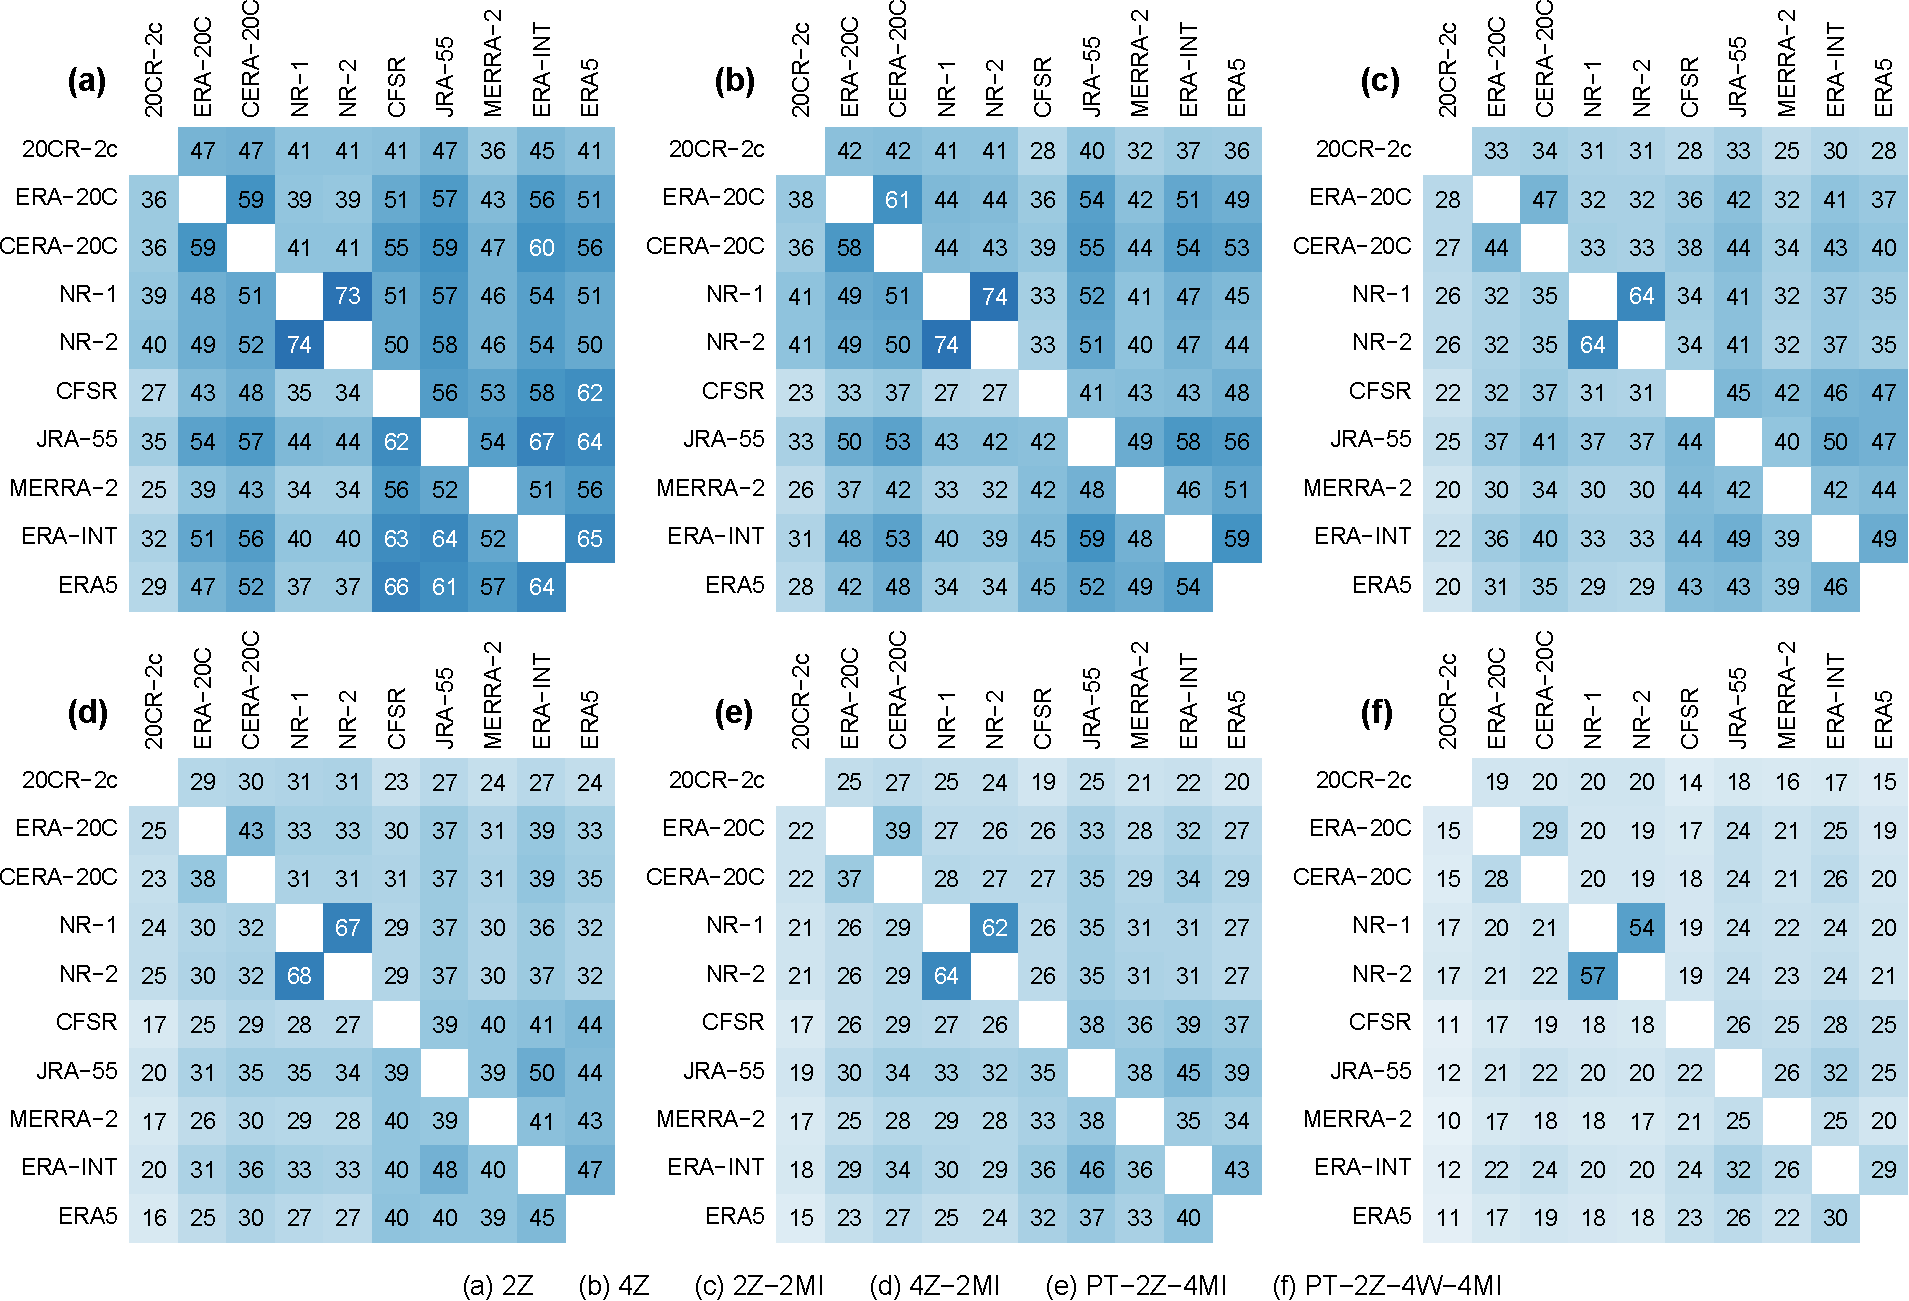
\includegraphics[width=120mm]{figures/similar-dates.pdf}
	\caption{Percentage of identical analogue dates selected when using the reanalysis datasets in columns that are also found when using the datasets in rows for different AMs. The values are averaged for all stations on the VP.}
	\label{fig:shared-dates}
\end{figure}

As it could be expected, ERA5 shared some similarities in the selection of analog dates with ERA-INT, but not in an order of magnitude that is really different from the other modern full-input reanalyses. Indeed, the percentage of shared analog dates is of the same order of magnitude as with CFSR and JRA-55, which are the two reanalyses produced by models with higher spatial resolution (Table \ref{table:datasets}), but fewer vertical levels. It is worth noting that JRA-55, which presents here strong similarities with ERA5 in terms of selected analog dates for Switzerland, has an output resolution that is five times lower (1.25\degree). However, JRA-55 shares more analog dates with ERA-INT than with ERA5. 


\section{Conclusions}
\label{sec:conclusion}

The choice of a reanalysis has a significant impact on the performance of AMs, as already shown in \citet{Horton2018b}. The influence of the dataset on the skill of the methods can even be larger than this related to the selection of the predictor variables. This has also been observed by other authors \cite{Dayon2015}. One of the conclusions of \citet{Horton2018b} is that the latest version of the full-input reanalyses should be used as they contribute to a better skill in the perfect prognosis context and for Switzerland, which is also likely valid for Europe. The subsequent release of ERA5 then raised the question of the potential benefit it could bring over ERA-INT, and to what extent the high spatial resolution could be informative for statistical downscaling.

This work focused on comparing ERA5 to the other main global reanalyses, and showed that it should be the dataset of choice for all tested AMs. Indeed, it surpassed the other reanalyses most of the time and was selected as the best dataset by about 50\% of the stations, and in on of the two first ranks by 75\% of the stations. Although ERA5 globally performed better than ERA-INT for the assessed AMs, ERA-INT was not systematically superseded by ERA5 for all stations. It it thus important to undertake such comparison with a large enough sample of stations in order to be capture well the overall picture. Even though ERA5 might not be the best reanalysis for all stations, it would not be advisable to patchwork the selection of reanalyses among stations. It would be recommendable however to use not a single, but a selection of reanalyses for certain applications.

ERA5 is distributed at very high spatial (0.25\degree) and temporal (1~h) resolutions. Although AMs are quick techniques, their calibration over several decades can be time consuming. This time increases all the more with a higher spatial resolution of the predictor grids. The high resolution even turned into a trap for the calibration technique here that ended up stuck in local minimas, resulting in poor skills. When using high resolution predictor grids, one should take care that the calibration technique used is able to satisfactorily optimize the spatial windows. The classic+ calibration \citep{Horton2019} could here successfully calibrate the spatial windows thanks to additional moves that allow it to go out of local minimas. \citet{Horton2018b} showed that below 1\degree, the gains are limited for AMs. ERA5 was tested at two resolutions here, its original one and the same resolution as ERA-INT (0.75\degree). The reduction in resolution did not impact the performance of AMs for daily precipitation, here mainly driven by synoptic-scale processes. This was shown not to be valid for predictands driven by mesoscale drivers. It also implies that the output resolution does not explain the gain in skill compared to ERA-INT, which are likely due to improvements in the forecast model, the assimilation scheme and the assimilated data.

To conclude, the use of ERA5 is recommended for the prediction of daily precipitation with AMs in Europe, ideally along with other reanalyses to provide an multi-model approach. However, for predictands that are primarily driven by synoptic-scale processes, using ERA5 at its full resolution is not justified and might even be dangerous if the calibration method does not handle it well.



\section*{acknowledgements}
Precipitation time series were provided by MeteoSwiss. The NCEP/NCAR, NCEP/DOE, and 20CR-2c were provided by the NOAA/OAR/ESRL PSD, Boulder, Colorado, USA, at http://www.esrl.noaa.gov/psd/. Support for the Twentieth Century Reanalysis Project dataset is provided by the U.S. Department of Energy, Office of Science Innovative and Novel Computational Impact on Theory and Experiment (DOE INCITE) program, and Office of Biological and Environmental Research (BER), and by the National Oceanic and Atmospheric Administration Climate Program Office. The CFSR, and JRA-55 were obtained from the CISL Research Data Archive (http://rda.ucar.edu/) at NCAR in Boulder, Colorado, and the NCAR is supported by grants from the National Science Foundation. The Climate Forecast System Reanalysis (CFSR) project is carried out by the Environmental Modeling Center (EMC), National Centers for Environmental Prediction (NCEP). The Japanese 55-year Reanalysis (JRA-55) project is carried out by the Japan Meteorological Agency (JMA). The MERRA-2 was obtained from the Goddard Earth Sciences Data and Information Services Center, Greenbelt, Maryland, from their website at http://disc.sci.gsfc.nasa.gov/mdisc. ERA-interim, ERA-20C, and CERA-20C were obtained from the ECMWF Data Server at http://apps.ecmwf.int/datasets/. ERA5 was obtained from the C3S climate data store (CDS) at https://cds.climate.copernicus.eu. Calculations were performed on UBELIX (http://www.id.unibe.ch/hpc), the HPC cluster at the University of Bern.


\section*{data availability}
All calculations were performed with the open source AtmoSwing software v2.1.1 \citep{Horton2019c}. The resulting files were processed using AtmoSwing R-toolbox v1.2.0 \citep{Horton2018d}.

The resulting analogue dates for every combination of station, reanalysis, and analogue method were published. These archives also contain different files: the parameter files used in AtmoSwing for the calibration, the resulting calibrated parameters, and files listing all assessed parameter sets. These files are available for ERA5 (...) and the other reanalyses \citep[see references in][]{Horton2018b}.

%TODO: publish data


\section*{conflict of interest}
The author has declared no conflict of interest.


% Here are examples of quotes and epigraphs.
%\begin{quote}
%The significant problems we have cannot be solved at the same level of thinking with which we created them.\endnote{Albert Einstein said this.}
%\end{quote}

%\begin{epigraph}{Albert Einstein}
%Anyone who has never made a mistake has never tried anything new.
%\end{epigraph}



%\printendnotes

% Submissions are not required to reflect the precise reference formatting of the journal (use of italics, bold etc.), however it is important that all key elements of each reference are included.
\bibliography{references}


\graphicalabstract{example-image-1x1}{Please check the journal's author guildines for whether a graphical abstract, key points, new findings, or other items are required for display in the Table of Contents.}

\end{document}
